\documentclass[twocolumn]{article}
\usepackage{graphicx}
\usepackage[utf8]{inputenc}
\usepackage[portuguese]{babel}
\usepackage{url}

\title{Trabalho 3 - Visão Computacional \\ \large Transformação Perspectiva}
\author{JOAO PEDRO VIEIRA SANTOS}
\date{\today}

\begin{document}

\maketitle

\begin{abstract}
Este trabalho apresenta o desenvolvimento de uma aplicação em Python e OpenCV para retificação de perspectiva em imagens de pinturas e fachadas arquitetônicas. O programa implementa o cálculo da homografia planar a partir de 4 pontos correspondentes, permitindo transformar imagens capturadas sob ângulos oblíquos em vistas frontais ortogonais. O código em \texttt{main.py} foi construído com suporte a interface interativa (via mouse) e modo automatizado em lote, incluindo funções para ordenação automática de vértices, estimativa euclidiana de proporções e realce de contraste por CLAHE. Os resultados práticos validam a restauração do paralelismo em três cenários de teste, e o projeto completo está disponível no Git.
\end{abstract}

\section{Introdução}
Fotografar quadros em museus ou fachadas prediais a partir de pontos de vista inclinados gera distorção projetiva: retas paralelas convergem para pontos de fuga e as proporções reais da obra são deformadas.

A transformação perspectiva (homografia 2D) permite reverter essa distorção. Conhecendo as coordenadas dos 4 vértices do plano na foto e definindo o retângulo de destino desejado, uma matriz $3 \times 3$ com 8 graus de liberdade é calculada para mapear os pixels de volta a uma visualização frontal canônica.

\section{O Que Foi Feito}
A aplicação foi implementada no arquivo \texttt{main.py} de forma modular, dividida nas seguintes etapas principais:

\subsection{Ordenação de Pontos (\texttt{ordenar\_pontos})}
Para que a transformação funcione de forma robusta e independente da ordem em que o usuário seleciona os cantos na imagem, a função organiza os 4 pontos em $[TL, TR, BR, BL]$ através de operações com suas coordenadas:
\begin{itemize}
    \item \textbf{Topo-Esquerdo (TL):} minimiza a soma $(x + y)$.
    \item \textbf{Fundo-Direito (BR):} maximiza a soma $(x + y)$.
    \item \textbf{Topo-Direito (TR):} minimiza a diferença $(y - x)$.
    \item \textbf{Fundo-Esquerdo (BL):} maximiza a diferença $(y - x)$.
\end{itemize}

\subsection{Estimativa de Dimensões (\texttt{calcular\_dimensoes\_destino})}
A função calcula a largura e altura do destino medindo as distâncias euclidianas dos lados opostos com \texttt{np.linalg.norm}, selecionando o maior valor entre topo/base e esquerda/direita. Isso preserva a escala original da cena e evita distorções por estiramento. Também há suporte para fixar proporções clássicas (como 4:3).

\subsection{Retificação (\texttt{retificar\_perspectiva})}
Com os 4 pontos de origem e os 4 cantos de destino $[(0,0), (W-1, 0), (W-1, H-1), (0, H-1)]$, a função:
\begin{enumerate}
    \item Calcula a matriz de homografia $\mathbf{H}$ através de \texttt{cv2.getPerspectiveTransform}.
    \item Aplica o mapeamento inverso de pixels com \texttt{cv2.warpPerspective}, utilizando interpolação bicúbica (\texttt{cv2.INTER\_CUBIC}) para máxima nitidez.
\end{enumerate}

\subsection{Pós-Processamento e Visualização}
O script inclui a função \texttt{realcar\_detalhes}, que converte a imagem para o espaço de cores LAB e aplica CLAHE no canal L para atenuar reflexos de iluminação em museus. Além disso, \texttt{desenhar\_anotacoes} e \texttt{criar\_painel\_comparativo} geram as imagens finais com os pontos numerados, o polígono demarcado e a visualização lado a lado (Antes $\times$ Depois).

\subsection{Modos de Execução da Aplicação}
O \texttt{main.py} possui dois modos de operação via linha de comando:
\begin{itemize}
    \item \textbf{Modo Interativo (\texttt{--interativo}):} gerido pela classe \texttt{SeletorInterativo}, abre a janela com \texttt{cv2.setMouseCallback} permitindo ao usuário clicar nos 4 cantos com o botão esquerdo. Teclas de controle: \texttt{'c'} para retificar, \texttt{'r'} para resetar, \texttt{'s'} para salvar em \texttt{output/} e \texttt{'q'} para sair.
    \item \textbf{Modo Demonstração (\texttt{--demo} ou padrão):} a função \texttt{executar\_experimentos\_batch} executa o pipeline automaticamente em 3 imagens de teste e salva os resultados em \texttt{output/}.
\end{itemize}

\section{Experimentos e Resultados}
Os experimentos foram executados pelo \texttt{main.py} e geraram os painéis comparativos e o arquivo \texttt{parametros\_experimentos.txt}:

\subsection{Cenário 1: Quadro a Óleo em Museu}
Foto oblíqua de um quadro com moldura nobre sob ângulo lateral ($\approx 35^\circ$). Os pontos selecionados foram $[(220, 180), (920, 110), (940, 630), (210, 520)]$. A retificação restaurou a vista ortogonal perfeitamente alinhada na dimensão $738 \times 553$ pixels (Figura~\ref{fig:museu}).

\begin{figure}[!ht]
    \centering
    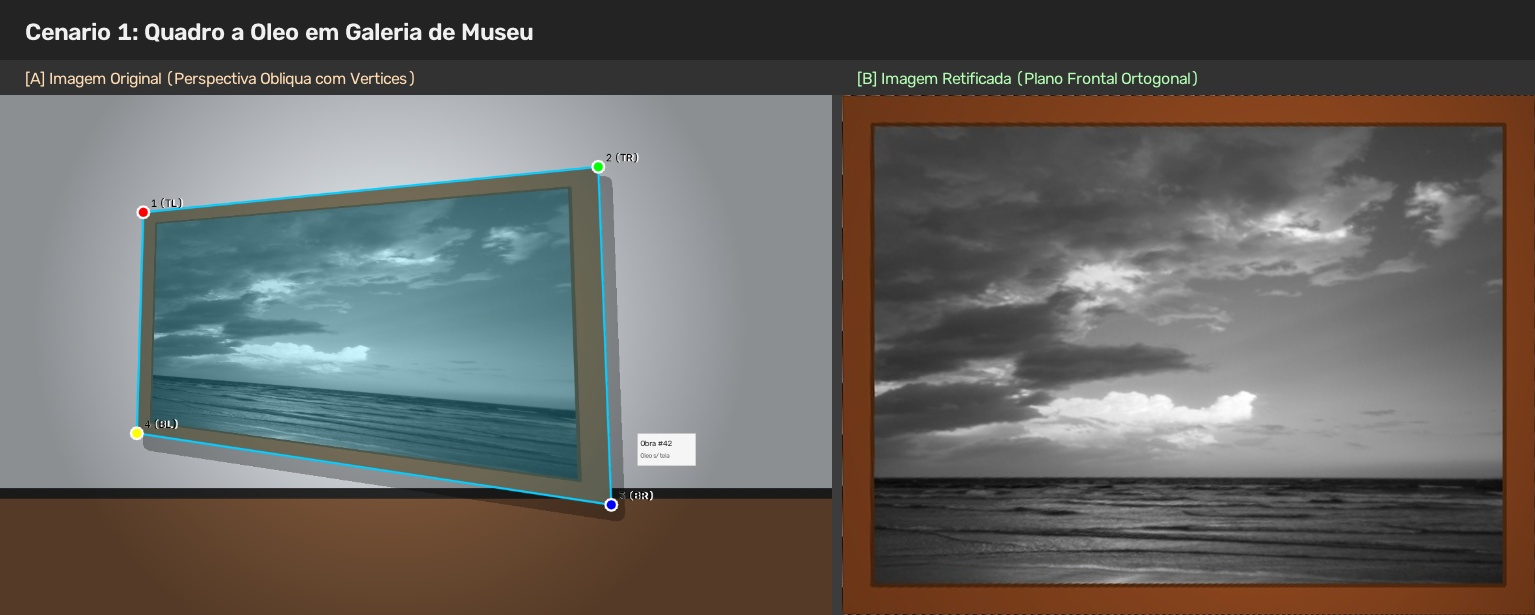
\includegraphics[width=\columnwidth]{output/cenario1_museu_comparacao.jpg}
    \caption{Cenário 1: Quadro a óleo em galeria antes e depois da retificação.}
    \label{fig:museu}
\end{figure}

\subsection{Cenário 2: Mural Urbano (Oxford VGG Graffiti)}
Mural na imagem clássica \texttt{graf3.png} sob forte perspectiva horizontal. Os 4 cantos da parede de tijolos foram corrigidos para o tamanho $520 \times 387$ pixels, restaurando as linhas de rejunte para a posição horizontal paralela (Figura~\ref{fig:grafite}).

\begin{figure}[!ht]
    \centering
    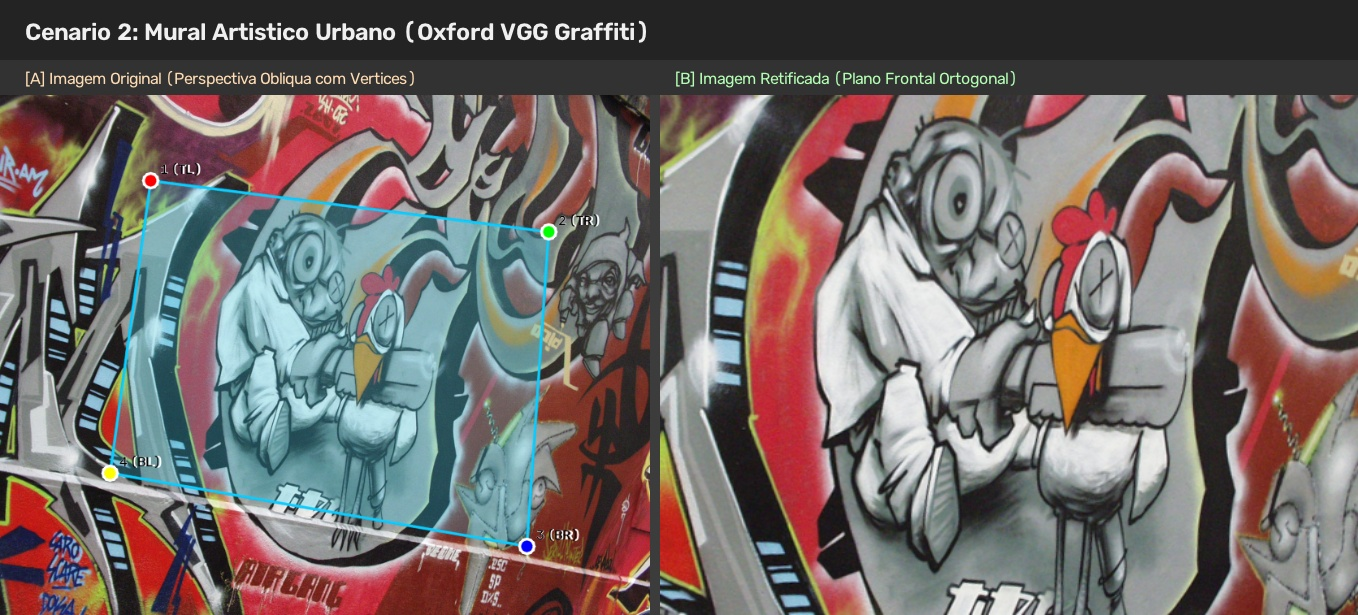
\includegraphics[width=\columnwidth]{output/cenario2_grafite_comparacao.jpg}
    \caption{Cenário 2: Retificação do mural artístico sobre parede de tijolos.}
    \label{fig:grafite}
\end{figure}

\subsection{Cenário 3: Fachada de Edifício}
Imagem \texttt{building.jpg} de uma fachada predial vista da rua. A transformação corrigiu a convergência vertical das colunas e janelas, gerando uma vista ortogonal plana de $315 \times 260$ pixels (Figura~\ref{fig:fachada}).

\begin{figure}[!ht]
    \centering
    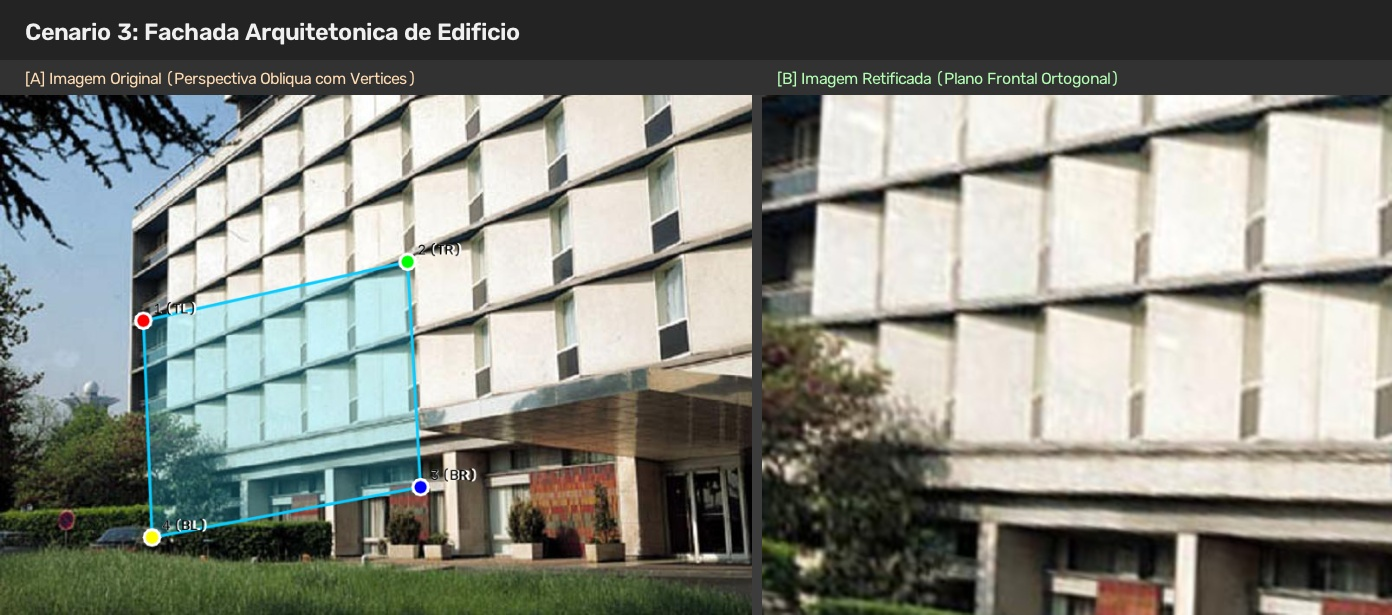
\includegraphics[width=\columnwidth]{output/cenario3_fachada_comparacao.jpg}
    \caption{Cenário 3: Fachada predial com restauração do alinhamento ortogonal.}
    \label{fig:fachada}
\end{figure}

\section{Conclusão}
A aplicação desenvolvida em \texttt{main.py} atingiu o objetivo proposto de retificação de perspectiva utilizando OpenCV. As funções de ordenação de pontos e estimativa de dimensões garantiram estabilidade e proporção geométrica correta às imagens retificadas, comprovando a utilidade da homografia planar em problemas de documentação de obras de arte e arquitetura.

\vspace{12pt}
\noindent\textbf{Link para o Código (Git):} \\
\url{https://github.com/JPeeeeee/visaoComputacional}

\end{document}
